\normaltrue
\correctionfalse

%\UPSTIidClasse{11} % 11 sup, 12 spé
%\newcommand{\UPSTIidClasse}{12}


\exer{Mouvement TT -- $\star$ \label{B2:13:03}}
\setcounter{numques}{0}
\UPSTIcompetence{B2-13}
\index{Compétence B2-13}
\index{Mécanisme à 2 translations}
\ifcorrection
\else
\textbf{Pas de corrigé pour cet exercice.}
\fi

\ifprof
\else
Soit le mécanisme suivant. On note $\vect{AB}=\lambda(t)\vect{i_0}$ et $\vect{BC}=\mu(t)\vect{j_0}$.
\begin{center}
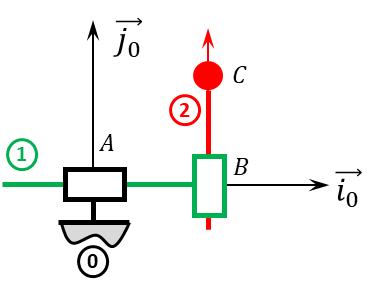
\includegraphics[width=.6\linewidth]{03_TT_01}
\end{center}
\fi

\question{Quel est le mouvement de \textbf{2} par rapport à~\textbf{0}.}
\ifprof
\else
\fi

\question{Donner l'équation horaire (trajectoire en fonction du temps) du point $C$ dans le mouvement de \textbf{2} par rapport à \textbf{0}.}
\ifprof
\else
\fi

On souhaite que le point $C$ réalise un cercle de centre $A$ et de rayon $R$. 

\question{Donner les expressions de $\lambda(t)$ et $\mu(t)$ permettant la réalisation de cette trajectoire à la vitesse $v=\SI{0,01}{m.s^{-1}}$.}
\ifprof
\else
\fi


\question{En utilisant Python, tracer $\lambda(t)$, $\mu(t)$ et la trajectoire générée.}
\ifprof
\else
\fi


\ifprof
\else
\begin{flushright}
\footnotesize{Corrigé  voir \ref{B2:13:03}.}
\end{flushright}%
\fi


